\section{LEARNING PROBLEM}
\label{sec:learning}

In the previous sections, we analyzed the optimal disclosure regimes under the assumption that the underlying environment parameters—specifically, the joint distribution of $(X, U, Y)$—are known to the Receiver. In this section, we transition from the decision problem to the learning problem, where the Receiver operates in an unknown environment. We consider two ways to pose the learning problem: static learning from a population sample and dynamic learning through repeated interactions.

\subsection{Static Learning}
\label{subsec:static_learning}
In the static learning setting, the Receiver is provided with a sample $\mathcal{D} = \{(x_i, u_i, y_i)\}_{i=1}^n$ containing $n$ i.i.d.\ observations drawn from the zero-mean joint distribution of $(X,U,Y)$. We assume the features and outcomes are bounded such that $\|X\|_\infty \le R$, $|Y| \le M$, $|U| \le M$, and the feature covariance matrix satisfies $\lambda_{\min}(\Sigma_{XX}) > 0$.

The population vanilla and strategic risks are given by:
\begin{align*}
R_V(q) &= \Var(Y) - (1-q)\Var(b_Y^\top X), &
b_Y &= \Var(X)^{-1}\Cov(X,Y), \\
R_S(b,q) &= \Var(Y) - (1-q)\E[G(X,Y)\Ind{F(X,U)>0}], &
G(X,Y) &= (2Y - b^\top X)b^\top X, 
\end{align*}
where $F(X,U) = (2U - b^\top X)b^\top X$, and the optimal strategic risk is $R_S^\star(q) = \min_b R_S(b, q)$.

The Receiver estimates these risks empirically. The vanilla risk $\hat{R}_V(q)$ is computed using the plug-in OLS estimator $\hat{b}_Y = \hat{\Sigma}_{XX}^{-1}\hat{\Sigma}_{XY}$. For the voluntary disclosure regime, the empirical strategic risk $\hat{R}_S(b,q)$ is the sample average of the strategic loss components $G_i \Ind{F_i > 0}$, and we denote its (regularized) empirical minimizer as $\hat{b}^\star$. We establish high-probability finite-sample bounds on the absolute estimation errors for both regimes.

\begin{theorem}[Finite-Sample Generalization Bounds]\label{thm:static_bounds}
For any $\delta \in (0, 1)$, with probability at least $1 - \delta$ over the random draw of $n$ samples, the empirical estimators satisfy:
\begin{align}
|\hat{R}_V(q) - R_V(q)| 
&\le \mathcal{O}\left( \frac{M^2 R^2}{\lambda_{\min}} \sqrt{\frac{d + \log(1/\delta)}{n}} \right), \label{eq:bound_vanilla} \\
|\hat{R}_S(\hat{b}^\star,q) - R_S^\star(q)| 
&\le \mathcal{O}\left( \left( M^2 + \|\hat{b}^\star\|_2^2 R^2 + \frac{\|\hat{b}^\star\|_2^4 R^4}{\lambda_{\min}} \right) \sqrt{\frac{d + \log(1/\delta)}{n}} \right). \label{eq:bound_strategic}
\end{align}
If the hypothesis class for the predictor weights is restricted to a bounded domain $\|b\|_2 \le B$, the norm $\|\hat{b}^\star\|_2$ in the strategic risk bound can be replaced by the deterministic constant $B$.
\end{theorem}

Since both estimators concentrate around their respective population risks, the empirical regret gap $|\hat{R}_S(\hat{b}^\star,q) - \hat{R}_V(q)|$ acts as a statistically sound proxy for the true strategic advantage. The triangular inequality yields the joint error bound:
\begin{equation}
    |(\hat{R}_S(\hat{b}^\star,q) - \hat{R}_V(q)) - (R_S^\star(q) - R_V^\star(q))| \le |\hat{R}_S(\hat{b}^\star,q) - R_S^\star(q)| + |\hat{R}_V(q) - R_V^\star(q)|.
\end{equation}
This confirms that whenever the empirical gap dynamically exceeds the composite $\mathcal{O}(1/\sqrt{n})$ error, selecting the empirically optimal regime mathematically aligns with the true Stackelberg equilibrium.

\begin{figure}[htbp]
    \centering
    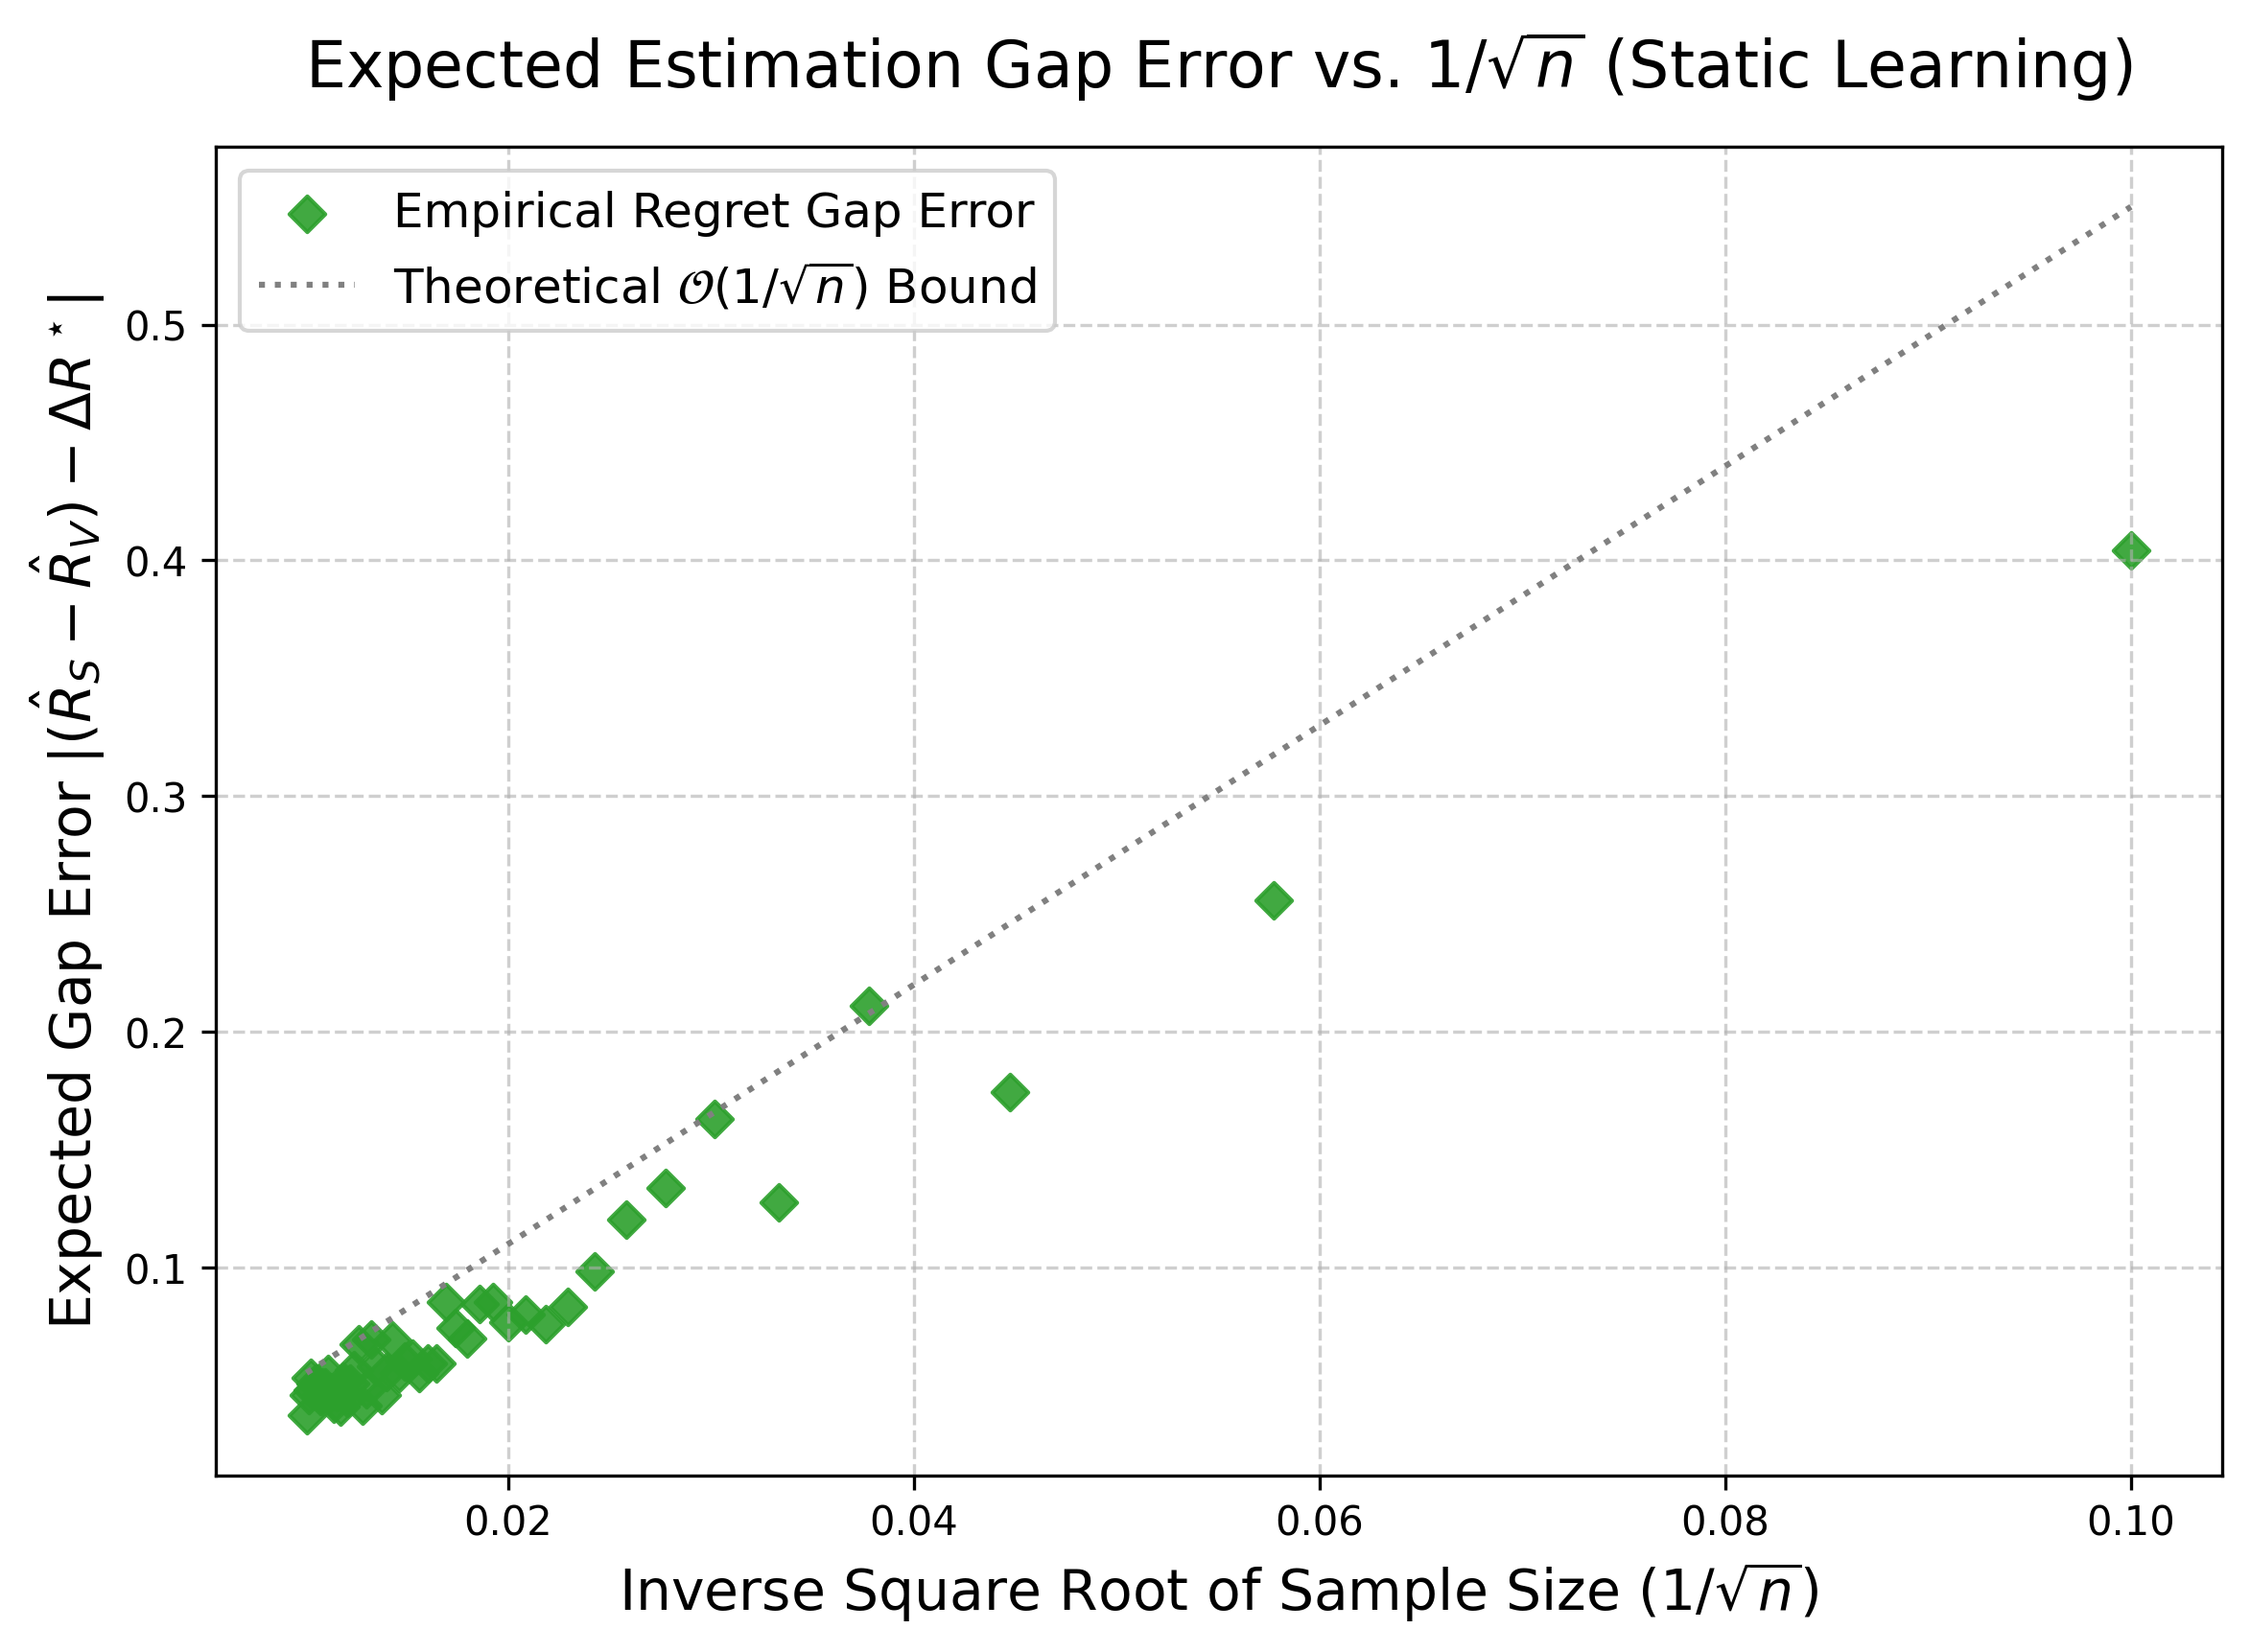
\includegraphics[width=0.6\linewidth]{figures/static_learning_gap_error.png}
    \caption{Simulated convergence of the empirical estimation gap error $|(\hat{R}_S - \hat{R}_V) - \Delta R^\star|$ as the sample size $n$ increases. Plotted against $1/\sqrt{n}$, the linear scaling confirms the $\mathcal{O}(1/\sqrt{n})$ rate derived in Theorem~\ref{thm:static_bounds}.}
    \label{fig:static_learning}
\end{figure}



\subsection{Dynamic Learning}
\label{subsec:dynamic_learning}
In the dynamic learning setting, the Receiver must learn the environment parameters over time through repeated interaction with the Sender. Consider a sequence of $T$ interactions. At each round $t \in [1, T]$, the Receiver selects a disclosure regime $D_t \in \{\text{Mandatory}, \text{Voluntary}\}$ and commits to a predictor $\hat{y}_t$. After the interaction, the Receiver incurs and observes the loss $\ell(y_t, \hat{y}_t(M_t))$.

The Receiver's objective is to minimize the cumulative regret $\mathcal{R}_T$:
\begin{equation}
    \mathcal{R}_T = \sum_{t=1}^T \ell\big(y_t, \hat{y}_t(M_t)\big) - T \cdot \min \{ R_V^\star, R_S^\star \}.
\end{equation}

\paragraph{Estimation Baseline.}
Before presenting the full algorithm, we establish the regret for a Receiver who a priori \emph{knows} the optimal regime. Even without having to learn the regime, the Receiver must still estimate the optimal predictor weights $b$ from sequential data.

\begin{lemma}[Estimation Regret Baseline]\label{lem:estimation_lb}
Suppose the optimal disclosure regime is known to the Receiver in advance. Using standard online optimization strategies under loss-only feedback, the expected regret from online estimation of the optimal predictor $\hat{y}^\star$ satisfies:
\begin{equation}
    \mathbb{E}[\mathcal{R}_T] \le \mathcal{O}(\sqrt{T}).
\end{equation}
\end{lemma}

The proof of Lemma~\ref{lem:estimation_lb} is provided in Appendix~\ref{app:online_learning}. This baseline result shows that the fundamental learning rate for estimating weights is $\mathcal{O}(\sqrt{T})$. This implies that if an adaptive algorithm can identify the regime quickly enough, its overall regret will still scale as $\mathcal{O}(\sqrt{T})$.

\begin{algorithm}[!ht]
\caption{Explore-Then-Commit (ETC) Disclosure Algorithm}
\label{alg:etc_disclosure}
\begin{algorithmic}[1]
\State \textbf{Input:} Time horizon $T$, exploration length $N$, confidence $\delta \in (0,1)$.
\For{$t = 1$ to $N$}
    \State Set $D_t = \text{Voluntary}$; predict $\hat{y}_t$ via current empirical estimate of $b$.
    \State Observe feedback $\ell_t$ and update empirical risks $\hat{R}_V$, $\hat{R}_S$.
\EndFor
\State \textbf{Switch Decision:} At round $N+1$, compare empirical risks.
\If{$\hat{R}_V \le \hat{R}_S$}
    \State Set $D_t = \text{Voluntary}$ for all $t \in [N+1, T]$.
\Else
    \State Set $D_t = \text{Mandatory}$ for all $t \in [N+1, T]$.
\EndIf
\For{$t = N+1$ to $T$}
    \State Predict using the committed regime; update online estimate of $\hat{y}^\star_{D_t}$.
\EndFor
\end{algorithmic}
\end{algorithm}

\begin{theorem}[Regret of the ETC Disclosure Algorithm]\label{thm:etc_regret}
Assume that $\Theta$ is compact and standard regularity conditions hold. The ETC Disclosure Algorithm (Algorithm~\ref{alg:etc_disclosure}) achieves sublinear expected regret:
\begin{equation}
    \mathbb{E}[\mathcal{R}_T] = \mathcal{O}(\sqrt{T}).
\end{equation}
\end{theorem}

\begin{figure}[htbp]
    \centering
    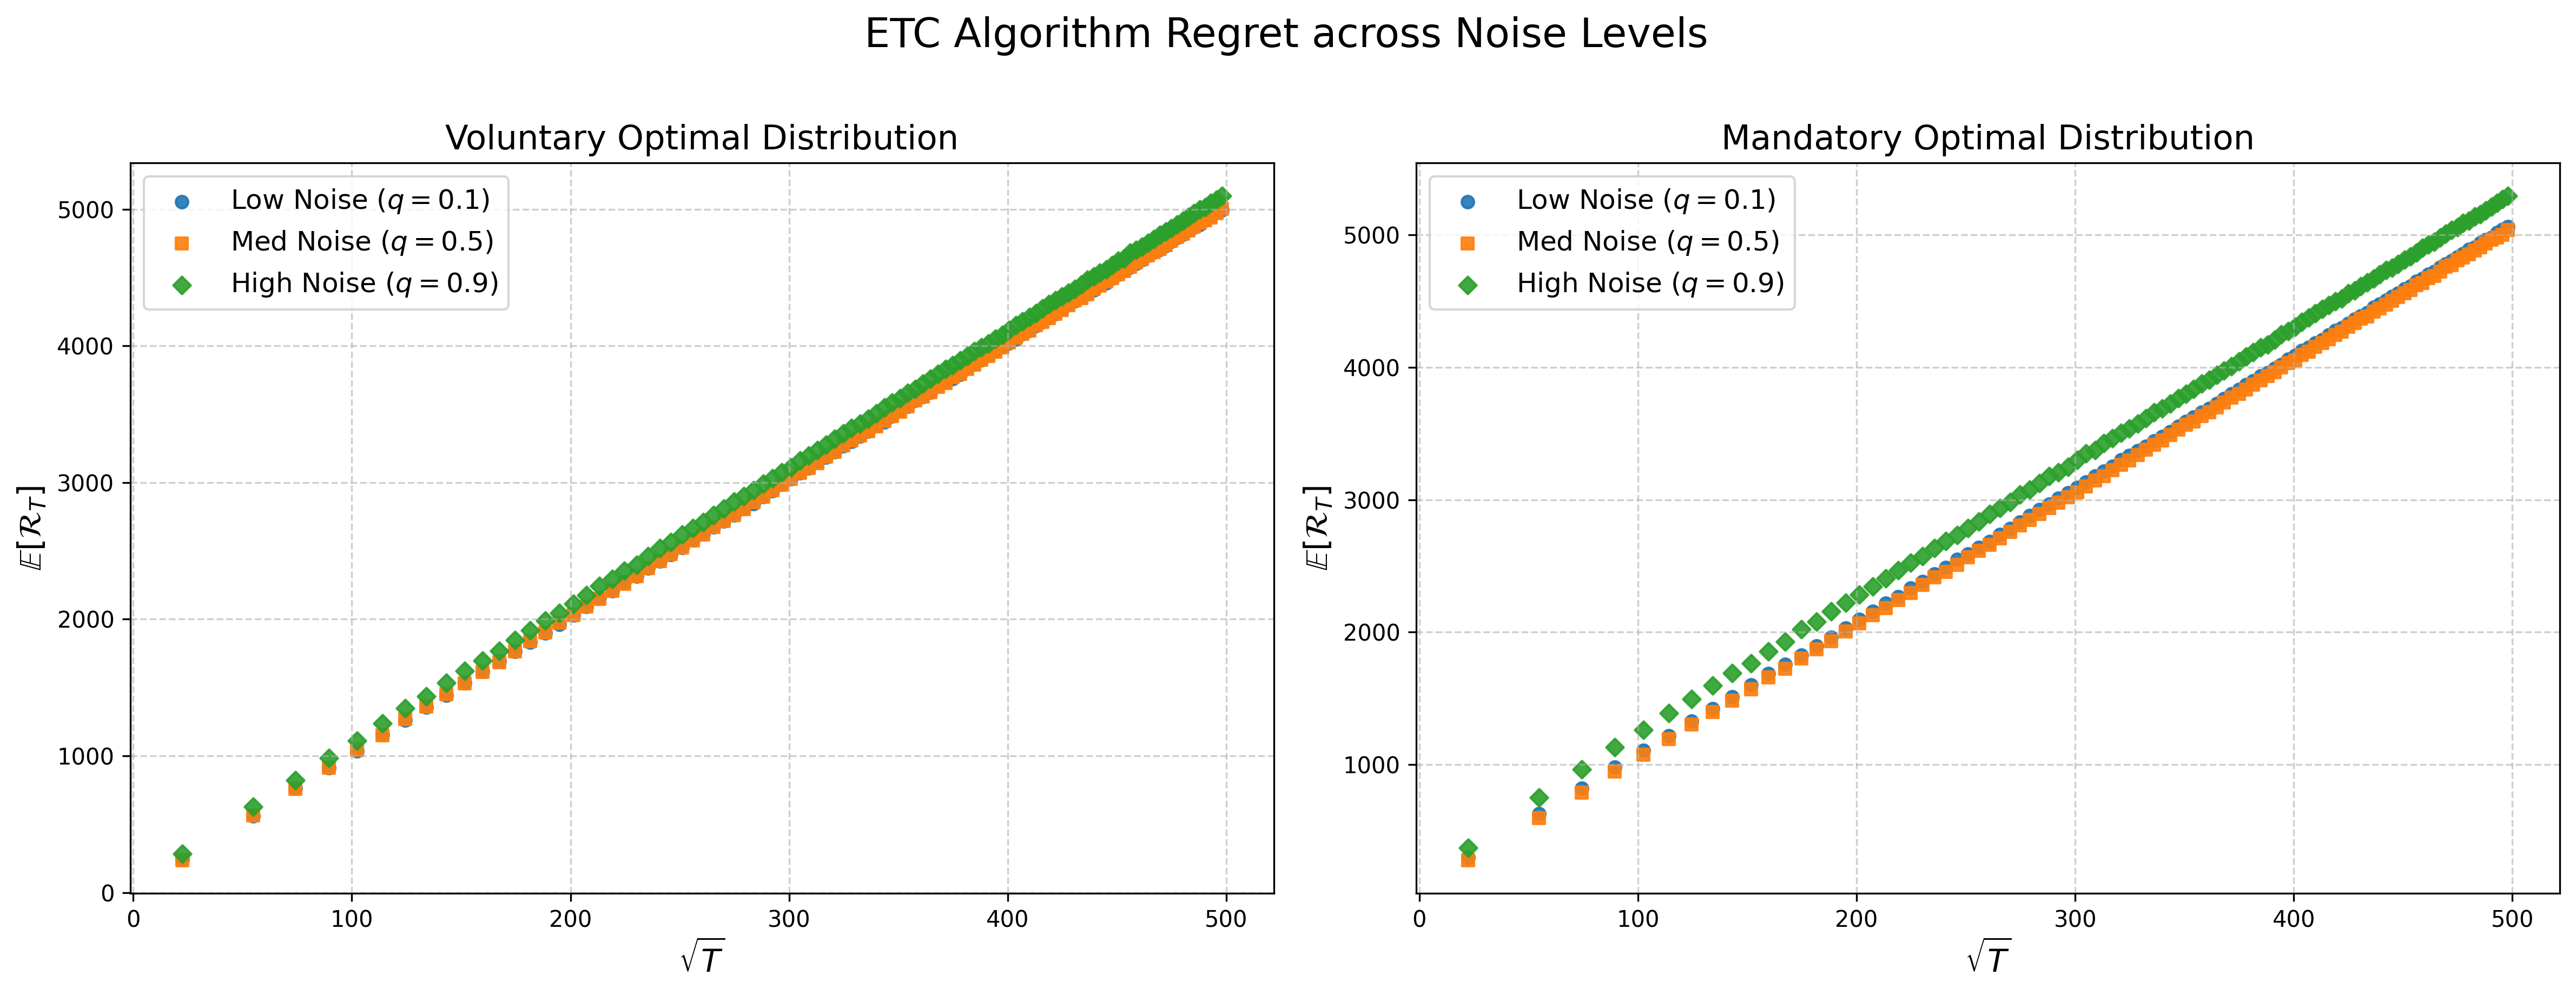
\includegraphics[width=\textwidth]{figures/dynamic_learning_regret.png}
    \caption{Cumulative expected regret $\mathbb{E}[\mathcal{R}_T]$ of the ETC Algorithm. The left panel shows an environment intrinsically favoring Voluntary disclosure, and the right panel shows an environment where feature-target misalignment makes Mandatory disclosure optimal. For each distribution, three noise levels ($q=0.1, 0.5, 0.9$) are plotted, showcasing tight tracking of the theoretical $\mathcal{O}(\sqrt{T})$ bounds across varying levels of information reliability.}
    \label{fig:dynamic_learning}
\end{figure}

